В конце прошлой лекции мы просветлились:
\begin{equation*}
	\left\{
	\begin{aligned}
		&\dot{n}_1 = - n_1 \sigma F + n_2 \sigma F + \frac{n_2}{\tau}\\
		&n_1 + n_2 = N
	\end{aligned}
	\right.
	\hspace{0.5 cm}
	\Rightarrow
	\hspace{0.5 cm}
	\dot{n}_1 = \dot{n}_2 = 0
	\hspace{0.5 cm}
	\Rightarrow
	\hspace{0.5 cm}
	\left\{
	\begin{aligned}
		&0 = - n_1 \sigma F + n_2 \sigma F + \frac{n_2}{\tau}\\
		&n_2 = N- n_1
	\end{aligned}
	\right.
\end{equation*}
Тогда в таком \textit{стационарном} приближении получаем:
\begin{equation*}
	n_1 = N \frac{F \sigma \tau +1}{1 + 2 F \sigma \tau},
	\hspace{1 cm}
	n_2 = N \frac{F \sigma\tau}{1 + 2 F \sigma \tau}.
\end{equation*}
Для изменения потока энергии (закон Гукера Ламберта Бэра) при прохождении через среду:
\begin{equation*}
	d F = F(\sigma n_2 - \sigma n_1) d z,
	\hspace{0.5 cm}
	F = F_0 \exp(- \alpha h),
\end{equation*}
где $h$ --- толщина образца.

\subsubsection*{Затемнение}
Пусть теперь у нас есть три уровня. С первого на второй и второго на первый: $\sigma_1$ и $\tau_1$. Со второго на третий и наоборот $\sigma_2$ и $\tau_2$.

\begin{figure}[h]
    \centering
    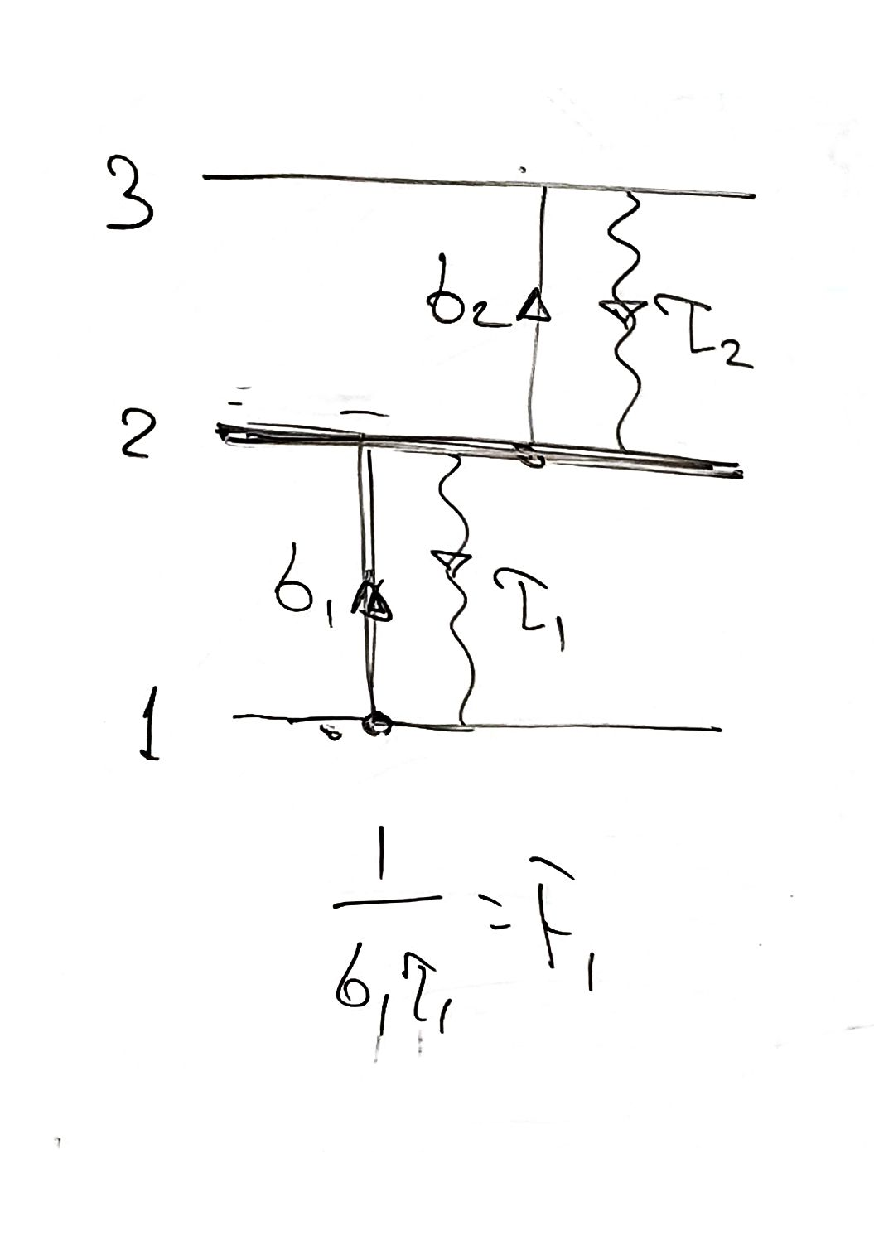
\includegraphics[width=0.3\textwidth]{img/zatemn.pdf}
    %\caption{}
    %\label{fig:}
\end{figure}


Запишем динамик нашей системы:
\begin{equation*}
\left\{
	\begin{aligned}
		&\dot{n}_1 = - n_1 \sigma_1 F + \frac{n_2}{\tau_1}\\
		&\dot{n}_2 = n_1 \sigma_1 F - n_2 \sigma_2 F - \frac{n_2}{\tau_1} + \frac{n_3}{\tau_2}\\
		&n_1 + n_2 + n_3 = N
	\end{aligned}
	\right.
\end{equation*}
Сразу работаем в стационарном приближении:
\begin{equation*}
\left\{
	\begin{aligned}
		&0  = - n_1 \sigma_1 F + \frac{n_2}{\tau_1}\\
		&0=n_1 \sigma_1 F - n_2 \sigma_2 F - \frac{n_2}{\tau_1} + \frac{n_3}{\tau_2}
	\end{aligned}
\right.
\hspace{1 cm}
\Rightarrow
\hspace{1 cm}
\left\{
	\begin{aligned}
		&n_2 = n_1 \sigma_1 \tau F = n_1 \frac{F}{F_1}\\
		&0= n_1 \sigma_1 F - \frac{n_2}{\tau_1} (\sigma_2 \tau_1 F +1)  + \frac{n_3}{\tau_2}
	\end{aligned}
\right.
\end{equation*}
Получаем выражение для $n_3$:
\begin{equation*}
	\frac{n_3}{\tau_2} =  \frac{n_2}{\tau_1} (\sigma_2 \tau_1 F +1)  - n_1 \sigma_1 F
	\hspace{0.5 cm}
	\Rightarrow
	\hspace{0.5 cm}
	n_3 = n_1 \sigma_1 \tau_1 \sigma_2 \tau_2 F^2 + n_1 \sigma_1 \tau_2 - n_1 \sigma_1 \tau_2 F = n_1 \frac{F^2}{F_1 F_2}.
\end{equation*}
В итоге получаем такую красоту:
\begin{equation*}
	n_1 + n_1 \frac{F}{F_1} + n_1 \frac{F^2}{F_1 F_2} = N.
\end{equation*}
Аналогично просветлению при проходе через среду:
\begin{equation*}
	d F = - (\sigma_1 n_1 + \sigma_2 n_2) F dz.
\end{equation*}
Если интегрировать можно увидеть качественно эффекты, которые далеки от реальности, однако дадут понимание. Здесь введен коэффициент поглощения: $\alpha(F) = \sigma_1 n_1 + \sigma_2 n_2$.

\begin{figure}[h]
    \centering
    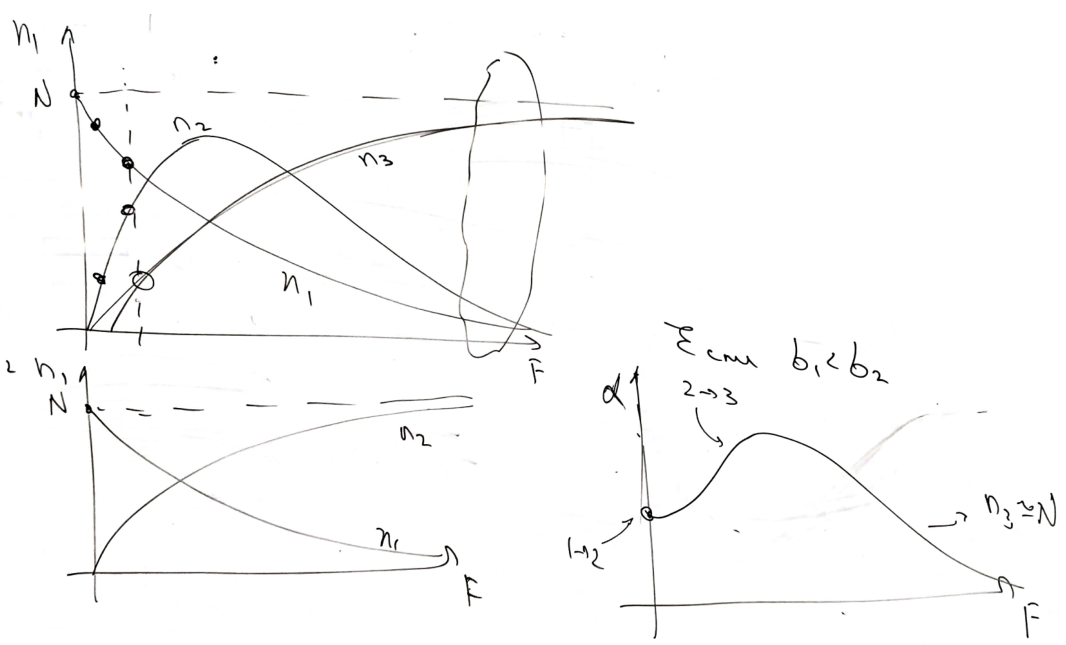
\includegraphics[width=0.7\textwidth]{img/konetz_zatemn.png}
    %\caption{}
    %\label{fig:}
\end{figure}

\subsubsection*{Теперь к лазеру}
Хочется, чтобы при облучении среда выдавала прибавку к излучению\footnote{это мне внезапно лень техать, так делать не надо.}: 

\begin{figure}[h]
    \centering
    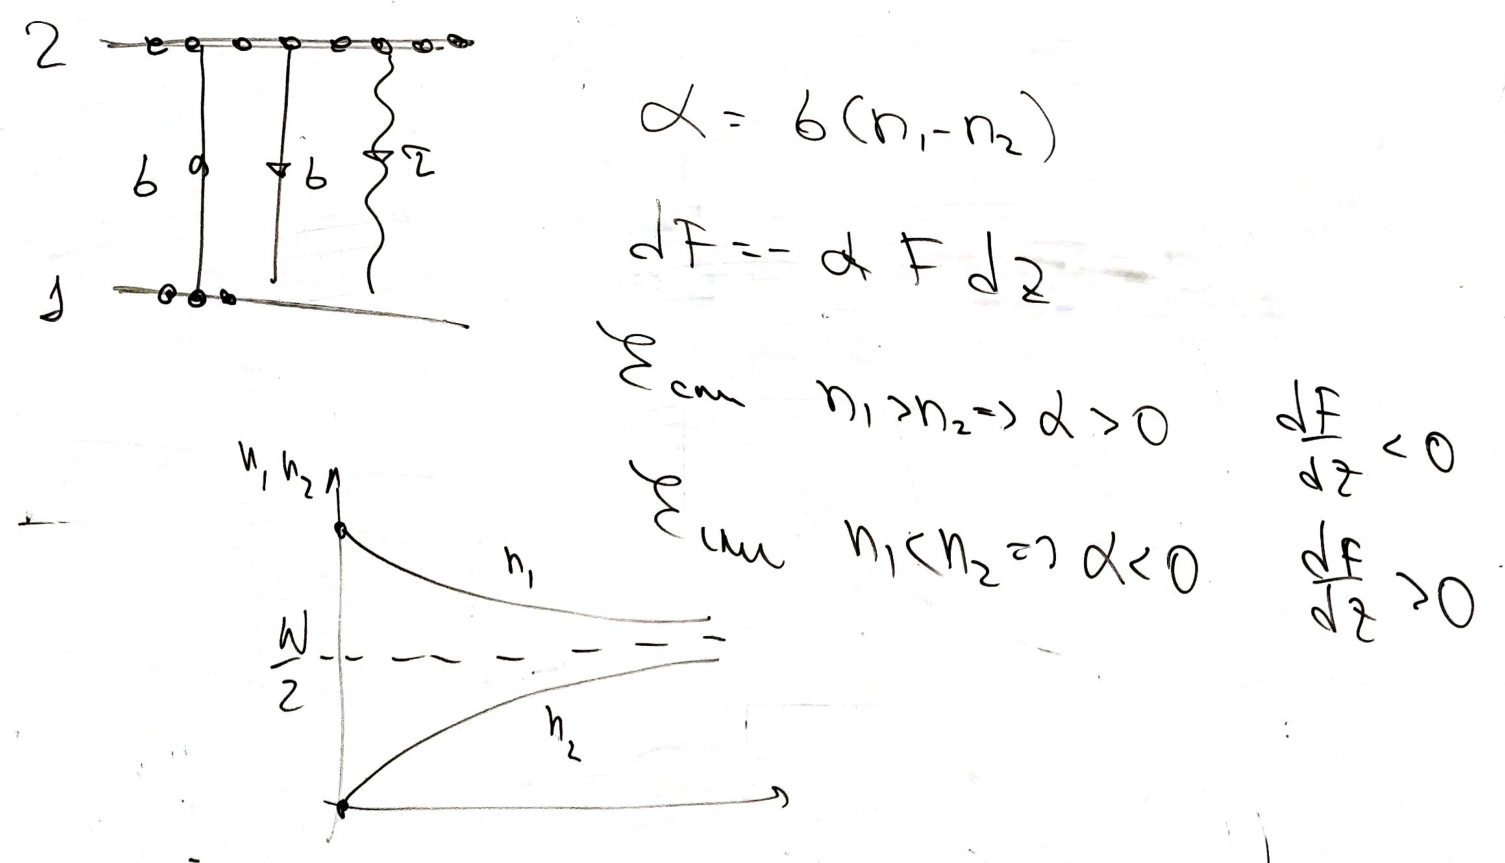
\includegraphics[width=0.8\textwidth]{img/len_texat1.png}
    %\caption{}
    %\label{fig:}
\end{figure}


Далее имеем другую систему, где вводим интенсивность накачки $W$ по забросу электронов с первого на второй уровень.

\begin{figure}[htb]
    \centering
    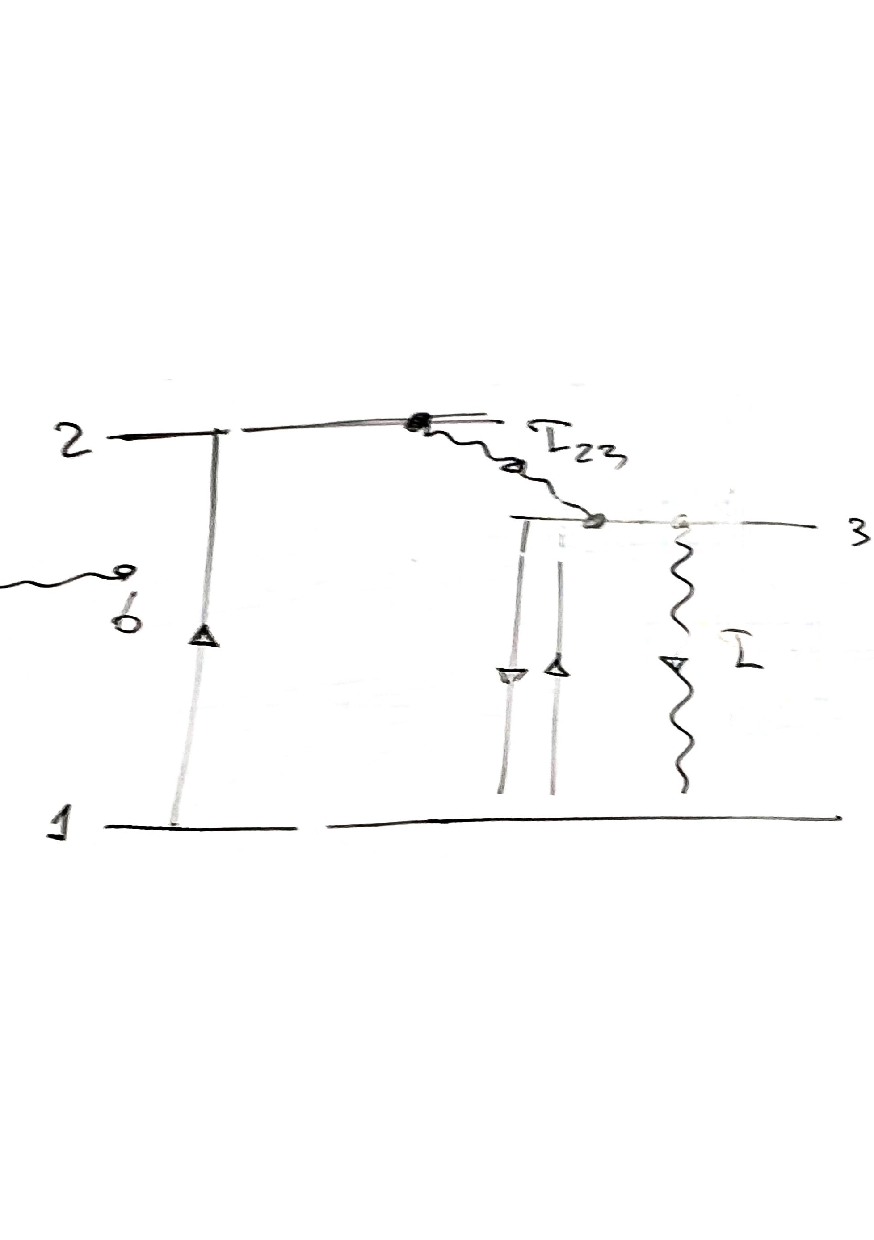
\includegraphics[width=0.3\textwidth]{img/2cxema.pdf}
     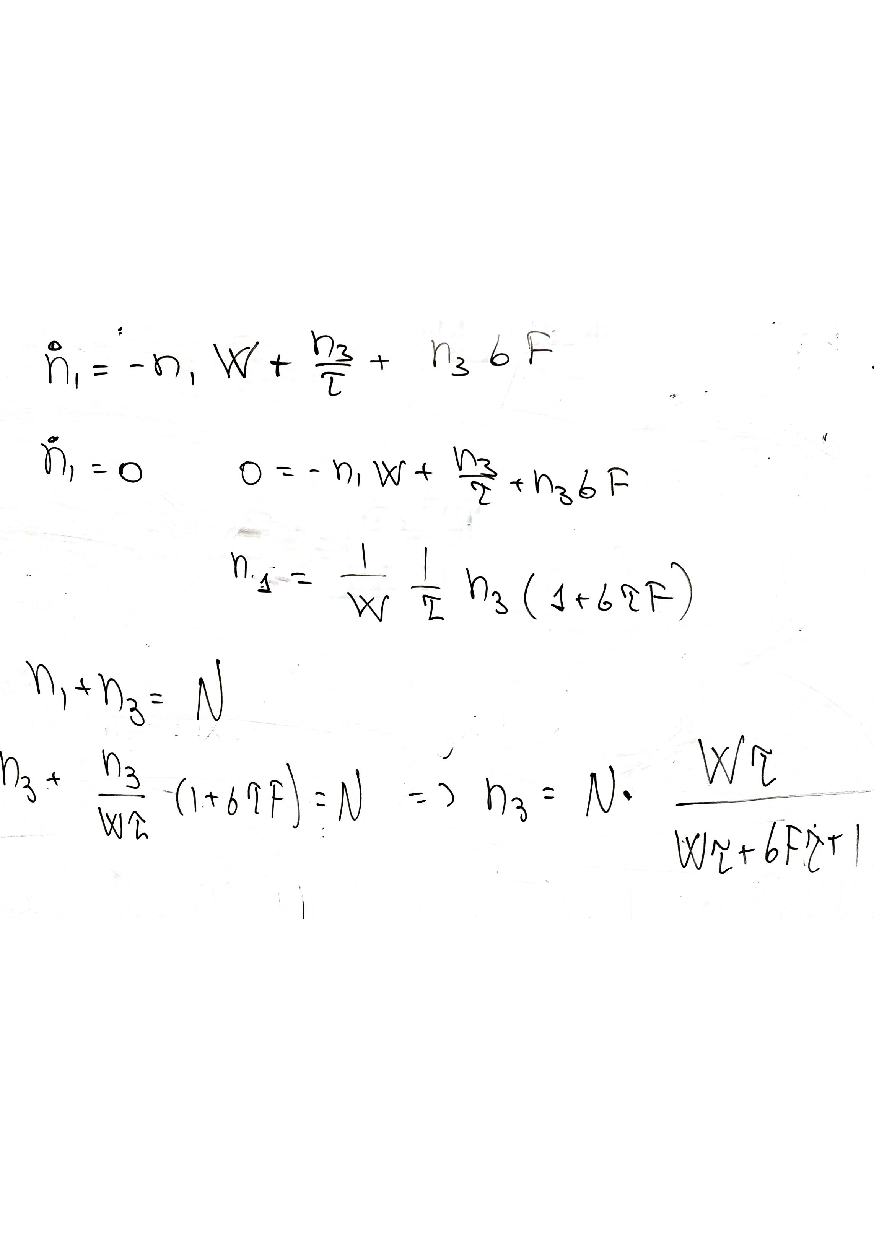
\includegraphics[width=0.3\textwidth]{img/len_texat2.pdf}
    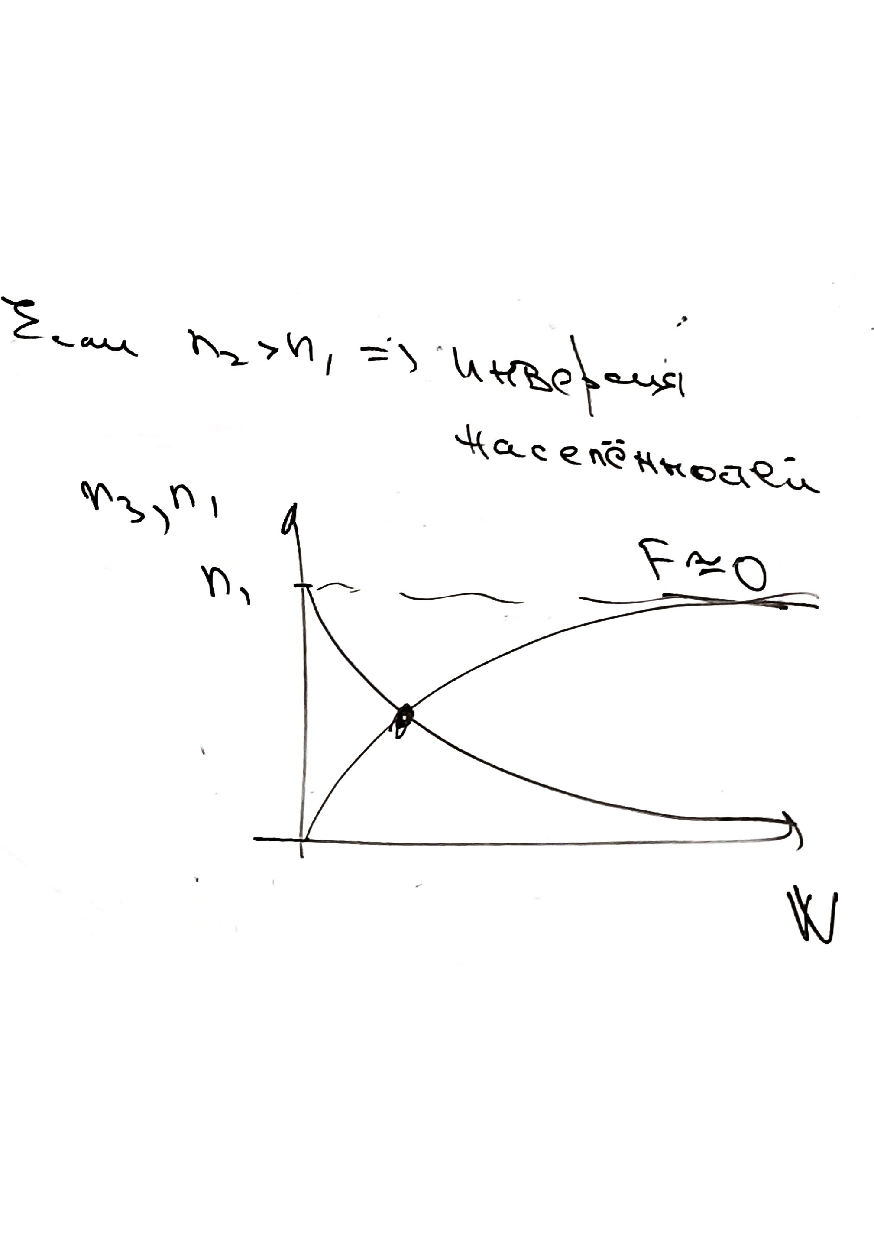
\includegraphics[width=0.3\textwidth]{img/inv_nas.pdf}
    %\caption{}
    %\label{fig:}
\end{figure}



Поставим изображенную среду между двумя зеркалами, и теперь из-за спонтанного свала электрона с третьего уровня нам может повезти и излучение от зеркала отразившись вновь вернется в среду и выбьет ещё один электрон и таким образом, за кучу итераций у нас возбудится нефиговый такой сигнал.
\begin{figure}[b]
    \centering
    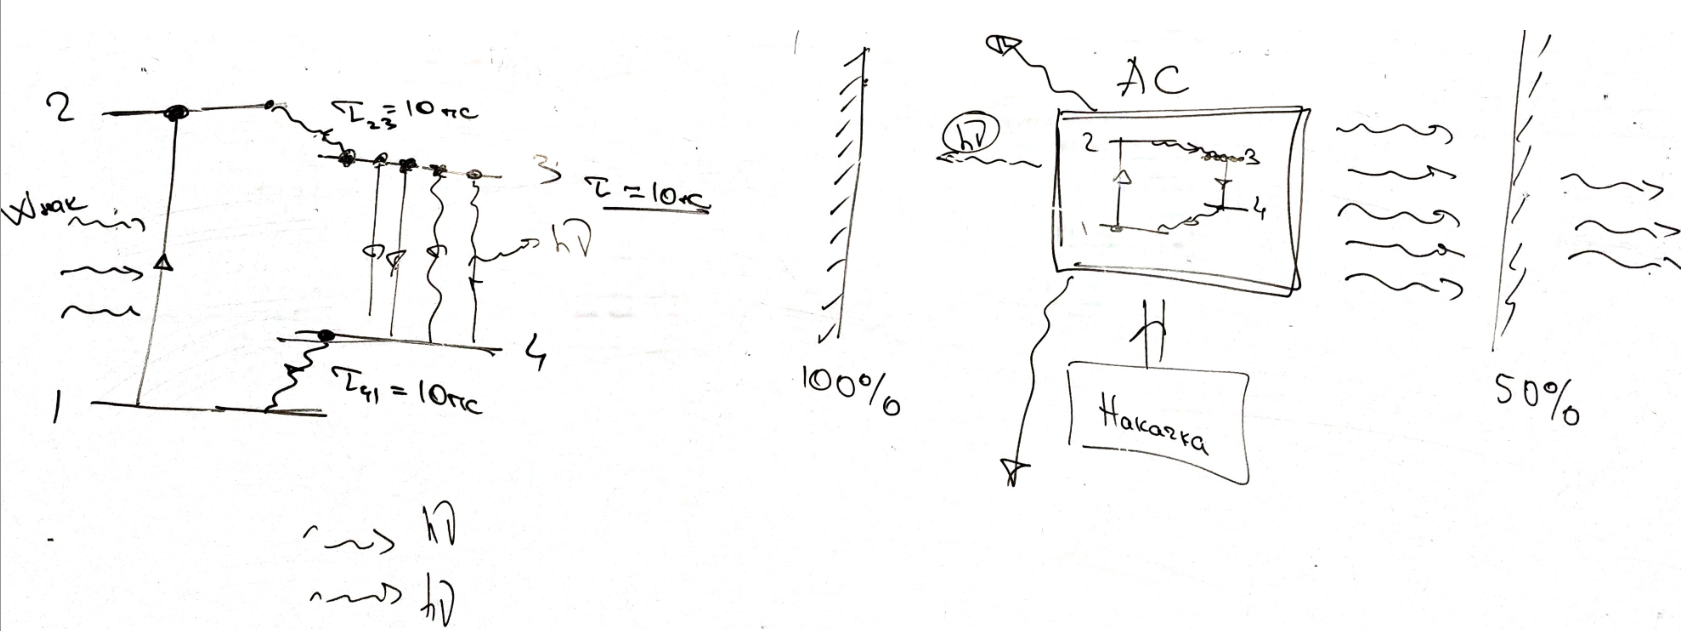
\includegraphics[width=0.8\textwidth]{img/3cxema.png}
    %\caption{}
    %\label{fig:}
\end{figure}

\begin{equation*}
	L = m \frac{\lambda}{2}
	\hspace{0.5 cm}
	\Rightarrow
	\hspace{0.5 cm}
	\lambda_m = \frac{2 h}{m}
	\hspace{0.5 cm}
	\Rightarrow
	\hspace{0.5 cm}
	\nu_m = \frac{c}{2 L} m.
\end{equation*}

И вот главная проблема, что даже при малых изменениях в системе (нагреве зеркал) у нас частота не будет совпадать с собственной возбуждения и ничего не срезонирует и не возбудится. 
Вспоминаем, что на прошлой лекции мы говорили про уширение, которое и позволит нам всегда попадать в резонанс, правда когда сделали такой лазер увидели, что слишком уж хорошо всё излучается, а хотелось бы монохроматичности вообще, а у нас продольные моды всякие гуляют. Кошмар!